\documentclass[a4paper, 10pt]{ctexart} %中文支持
\usepackage{float}              %防止浮动元素浮动
\usepackage{rotating}           %旋转图片
\usepackage{amsfonts}           %对某一些字体之支持
\usepackage{mathrsfs}           %mathscr e.g.
\usepackage[]{amsmath}          %数学公式
\usepackage{amsthm}             %定义, 定理, 证明, 例子环境的支持
%使用方法:
%\newtheorem{environment name}{caption}
%比如 \newtheorem{example}{这是例子}
%效果 \begin{example} xxx \end{example} -> 这是例子 1 xxx
%proof就不需要了
\usepackage{graphicx}           %插入图片
\usepackage[left=1.25in,right=1.25in,top=1in,bottom=1in]{geometry}   %用来排版的
\usepackage[]{color}            %给部分文本上色的
\usepackage{algorithm}          %写伪代码的
%\usepackage{algorithmic}       %同上
\usepackage{algorithmicx}
\usepackage{algpseudocode}
\usepackage{minted}
\usepackage{amssymb}            %用来加入一些数学符号, 比如说 $\varnothing$
\usepackage{titlesec}
\usepackage{fontspec}           %不知道用来干嘛的
\usepackage{hyperref}           %生成可跳转的书签
% -------------------------------
\setmonofont{Ubuntu Mono}       %?
\usemintedstyle{custommanni}    %设置minted插入代码的风格
\titleformat*{\section}{\huge\bfseries}             %管理title的字体和大小
\titleformat*{\subsection}{\Large\bfseries}         %bfseries就是默认的字体.
\titleformat*{\subsubsection}{\large\bfseries}
% -------------------------------
\newtheorem{theorem}{Theorem}
\newtheorem{example}{Example}
\newtheorem{definition}{Definition}
\newtheorem{lemma}{Lemma}
\newtheorem{remark}{Remark}
\newtheorem{corollary}{Comment}
\newtheorem{proposition}{Proposition}
\pagestyle{plain}

\title{chapter 4}
\author{ You \and me}
\date{Yesterday}
\begin{document}
\maketitle
\tableofcontents
\section{引入}
\subsection{what is Fibonacci sequence}
the definition of Fibonacci sequence is well-known. Let's say $F \left(n\right) $ stands for the
n th member of Fibonacci sequence. We have that 
\begin{align*}
    F\left(n\right) = 
    \begin{cases}
        1 & n  =1 \\ 
        1 & n  = 2 \\
        F\left(n  -1\right) + F\left(n  -2\right)& n > 2 \\
    \end{cases}
\end{align*}
I can write some code now. 

\begin{minted}{c++}
public int fib (int n) {
    if (n < 1) {
        return -1;
    }
    if (n == 1 || n == 2) {
        return 1;
    }
    return fib(n-1) + fib(n-2);
}
\end{minted}
we can see that the time complexity of the algorithm is  $O \left( 2^{n}\right)$. 
And why is that happening? Can we do better? Because, when we are calculating the 
Fibonacci sequence, we don't seem to need that much time.

\subsection{what is dynamic programming}
动态规划的前提实际上和我们的递归解法什么的是类似的, 都需要有递归的子结构.
\begin{quotation}
    动态规划 = 分治递归+记忆储存
\end{quotation}
和分治递归之间的区别就是在于这个记忆储存, 因为分治递归的过程中, 
部分子问题会被重复求解, 
我们将子问题的解储存下来, 以此来提高效率.
\begin{example}
    斐波那契数列的求解过程中, 子问题会被重复求解. 
    
    比如说我现在给出一个求斐波那契数列中, 某一项值的递归函数.

    \[
    F(n) = 
    \begin{cases}
        1& ,  n =1  \\ 
        1 & , n=2  \\
        F\left(n-1\right) + F\left(n-2\right)& , n>2
    \end{cases}
    \]

    \begin{figure}[H]
        \centering
        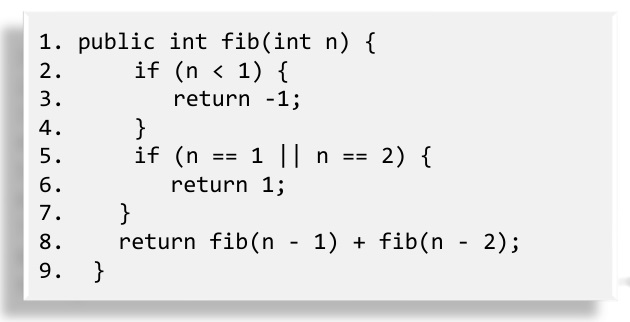
\includegraphics[scale = 0.5]{1.jpg}
    \end{figure}

    我们看到这里的时间复杂度非常高, 有 $O\left(2^{n}\right)$, 是非常糟糕的算法.\footnote{怎么求出来的?}
    但是我们自己手算的时候体感并没有那么夸张, 这是因为这个函数重复求解了很多子问题

    为此我们可以画一颗树:
    \begin{figure}[H]
        \centering
        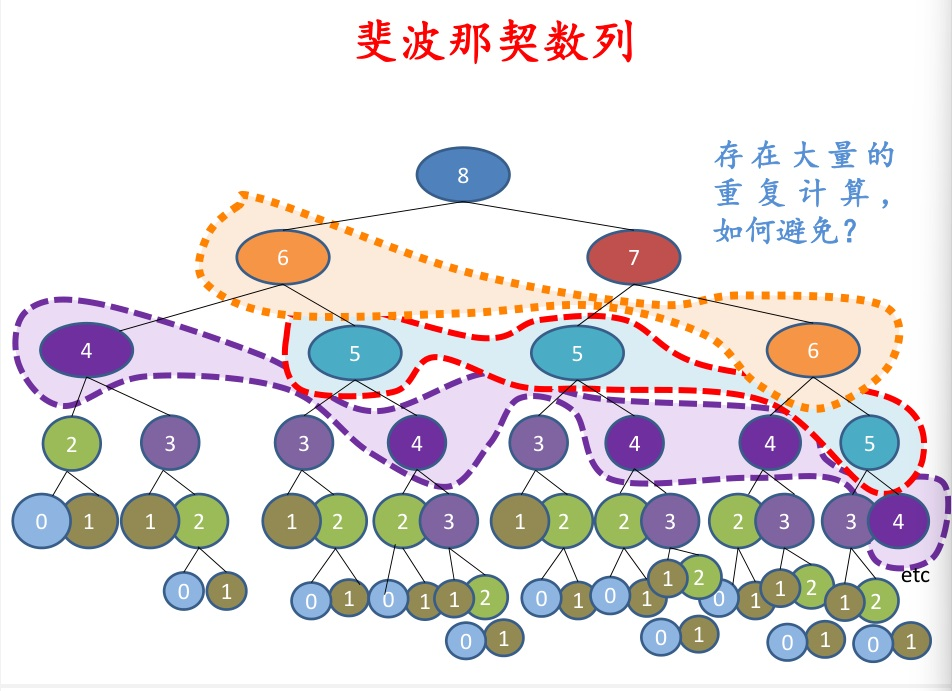
\includegraphics[scale = 0.3]{2.jpg}
    \end{figure}

    这边圈出的都是重复计算的, 数量比较夸张, 这种重复求解子问题的情况,
    就是动态规划适用的时候.
\end{example}

\section{动态规划的一些基本原理}

分治法的特点
\begin{quotation}
    1.子问题是相互独立的

    2.如果说子问题之间不是相互独立的, 分治方法将会重复计算子问题, 效率很低
\end{quotation}

the dynamic programming is a paradigm or an approuch, which is not a 
specific algorithm to solve certain problems.

Divide and conquer has no memory. It is stupid. The same questions are 
being solved over and over again (in some situation). It works fine if we 
the subproblems are independent (as what we mention previously).

So what is dynamic programming? In a simpliest way, it can be described as follows:
\begin{enumerate}
    \item It is the improvement of divide and conquer.
    \item It need memory
    \item The memory is a list. The solution of subproblems are stored in the 
    list.
    \item We start from the smallest subproblem.
\end{enumerate}


The dynamic programming is used only when:
\begin{enumerate}
    \item[-] we have 优化子结构
    \begin{enumerate}
        \item[·]一个问题具有优化子结构, 如果其优化解包含了子问题的优化解.
        \item[·]缩小子问题的集合, 我们只要优化问题中的子问题, 以此降低复杂性
        \item[·]优化子结构使得我们能够自下而上地完成求解  
    \end{enumerate}
    \item[-] and we have 重叠子问题
    \begin{enumerate}
        \item[·]子问题的解被多次使用
    \end{enumerate}
\end{enumerate}

\begin{figure}[H]
    \centering
    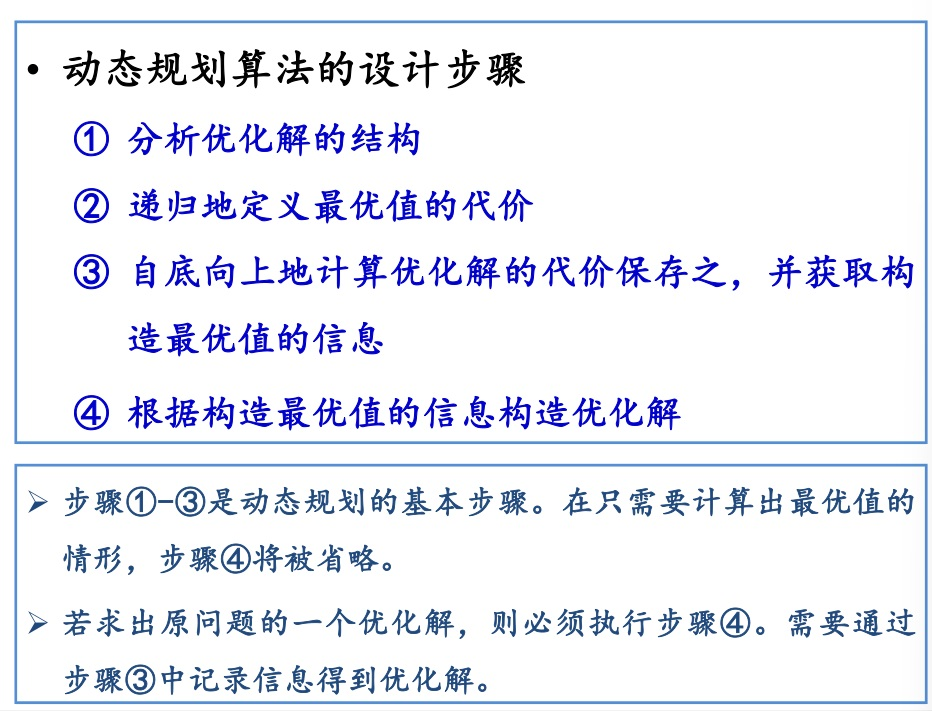
\includegraphics[scale  = 0.5]{5.jpg}
\end{figure}

看了不一定有什么概念, 接下来我们给出实例.
\section{矩阵链乘法问题}
在矩阵乘法中, 我们适当使用结合律是能提高效率的. 
为此, 我们应当加上适当的括号, 使得所用时间最少.
\begin{example}
设 
$A_1 \in \mathbb R ^{10 \times 100}, 
A_2 \in \mathbb R ^{100 \times 5} , 
A_3= \mathbb R ^{5 \times 50}$
我们计算 $A_1 \times A_2 \times A_3$, 我们能够发现, 
$\left(A_1 \times A_2  \right) \times A_3 $ 以及 $A_1 \times \left(A_2 \times A_3\right)$
的代价\footnote{就是花费的步骤, 操作的次数}是不一样的.

前者是 $10 \times 100 \times 5 \times 100 \times 50 \times 5$, 后者是 $100 \times 5 \times 50 \times 10 \times 100 \times 50$
\footnote{$A \in \mathbb R ^{p\times q } , B \in 
\mathbb{R} ^{q \times r}\implies$ 代价为 $O\left(pqr\right)$, 不妨证明一下}

So we have the conclusion that the multiplication between matrices suit 结合律.
But the different parenthesis may contribute to 
different cost.
\end{example}
\subsection{问题描述}
\noindent What we going to do is to find 
the smallest cost that the multiplication makes and 
find how the parenthesis is distributed, if possible.
现在给出准确的定义

\noindent \textbf{Input:} 给定 $n$ 个矩阵 
记为 $\left\{A_n\right\}$ \\
\textbf{Output:} 给出最优的效率, 以及其划分

试着使用穷举. 设 $p\left(n\right)$ 是计算 $n$ 个矩阵相乘的方法数目.
设其最外面两个的括号是这样的 $\left(A_1 \times A_2 \times \cdots  \times A_k \right) \times \left(A_{k+1} \times \cdots  \times A_n\right)$
就有
\[
p\left(n\right) 
= \sum_{k=1} ^{n-1} p\left(k\right) p(n-k) 
\footnote{这里为什么是 $n-1$ 捏, apparently it is pointless to have something like $\left(A_{1 } \times A_{2}\right)$, the parenthesis is nonsense.}
\]
其中 $n > 1$, $p(1)$ 定义为 $1$

这里有个结论: 满足上面这个递推式的数字称为卡特兰数字\footnote{这是计算机领域和组合(应该)中经常出现的}, 记为 $C$
\[
\begin{aligned}
    p\left(n\right) & = C\left(n-1\right) = \frac 1n \binom{2\left(n-1\right)}{n-1} = \frac{\big( 2\left(n-1\right) \big) !}{n! \left(n-1\right)!}\\
    & = \Omega \left( 4 ^{n} / n ^{3 /2}\right) \footnotemark
\end{aligned}
\]
\footnotetext{这是tm怎么来的}
\subsection{分析优化解的结构}
假设矩阵链应当在 $k$ 处断开, 得到两个子链 $A_i \times \cdots  \times A_{k}, A_{k+1} \times \cdots  \times A_{j}$.
\begin{theorem}
    如果确定了上面两个子链的优化顺序, 则确定原矩阵链的优化顺序
\end{theorem}
\begin{proof}
    反证法, 原矩阵链的优化顺序可以拆为两段, 分为对应两个子链. 记为 $A =U \times V$\footnotemark
    设子链的优化顺序为 $U_{0} , V_0$ (这是已知条件) , 我们要证明的是 $U_0 \times V_0$ 和 $U \times V$ 等价\footnotemark.

    如果说不等价, 设 $U_0< U$, 那么 $U_0 \times V$ 比 $U \times V$ 更优的顺序. 矛盾
\end{proof}
\footnotetext[8]{这个符号我尽力了}
\footnotetext{突然冒出来的``等价''是为了严谨}
如图, 有重叠子问题, 所以说可以使用动态规划
\begin{figure}[H]
    \centering
    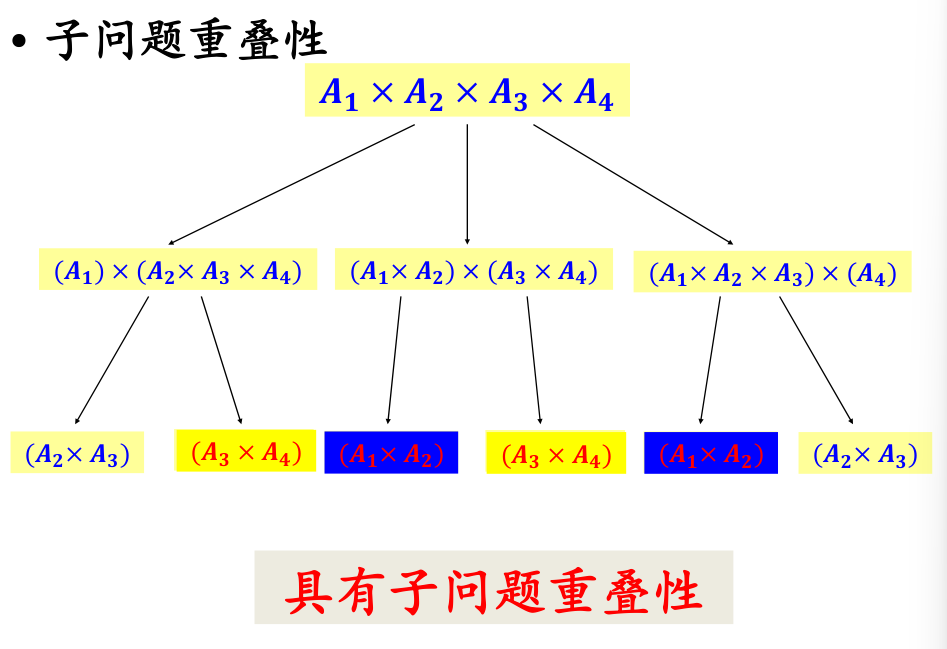
\includegraphics[scale = 0.5]{6.png}
\end{figure}

\subsection{递归地定义最优值的代价}
\begin{definition}
设 $A_i \in \mathbb{R} ^{p_{i-1}\times p_{i}}$, 序列 $\left\{ p_{i}\right\}, i = 0, 1 , \cdots  , n$ 表示矩阵的列或者行\\ 
\end{definition}
\begin{definition}
设 $m [i, j ]$ 是计算 $A_{i \sim j}$ 的最小乘法数. 有:
\end{definition}
\[
    m\left[ i,j  \right]= 
    \begin{cases}
        \displaystyle \min_{i\le k <j} \left\{ m[i , k] + m [k+1 ] + p_{i-1} p_k p_j\right\} & i < j\\
        0 & i = j 
    \end{cases}
\]

我们可以将 $m$ 视作一个矩阵, 对角线上的元素已知, 自底向上地计算. 
\subsection{计算代价}
\begin{figure}[H]
    \centering
    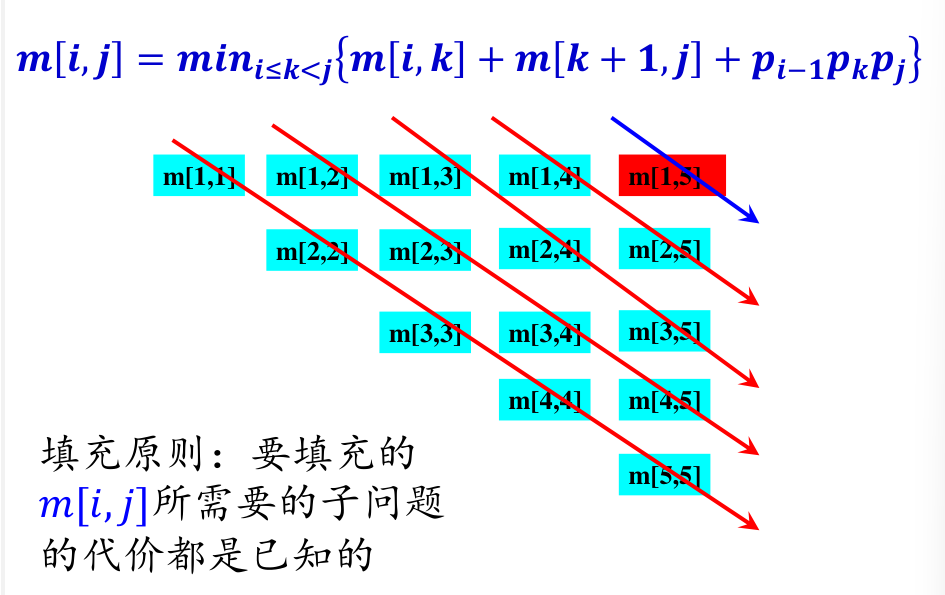
\includegraphics[scale =0.5]{7.png}
\end{figure}
\subsection{伪代码}
\begin{figure}[H]
    \centering
    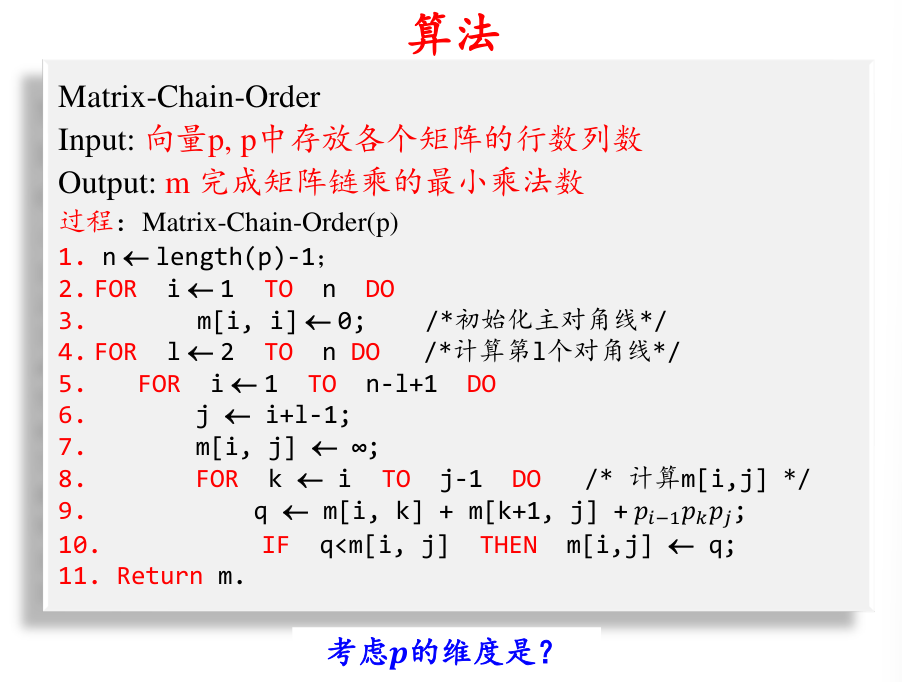
\includegraphics[scale =0.5]{8.png}
\end{figure}

\begin{minted}{c++}
int main (){
    // let's say that we count from 0
    int n = length of array;
    for (int i = 0 ; i < n ; i++){
        m[i][i] = 0;
    }
    int min = 100000;
    for (int i = 0 ; i < n ; i ++){
        for (int j =1 ; j < n - 1 ;j ++ ){
            min = 10000;
            for (int k = i ; k < j + 1 ; j++){
                if (i+j && min > m[i][k]+m[k+1][i+j]+p[i-1]p[k]p[i+j]){
                    min = m[i][k]+m[k+1][i+j]+p[i-1]p[k]p[i+j];
                }
            }
            m[i][j] = min;
        }
    }
}
\end{minted}
\subsection{获取构造最优解的信息}
How to store the position of parenthesis? apparently, we have to write down the k above when the for block
of k stop exercuting. That is not difficult.

用矩阵 $S$ 来储存最优的划分处, $S \left[ i, j  \right]$ 就是储存了最优的划分 $k$ , 分为 $A_{i \sim k}, A_{k+1 \sim j}$
\begin{figure}[H]
    \centering
    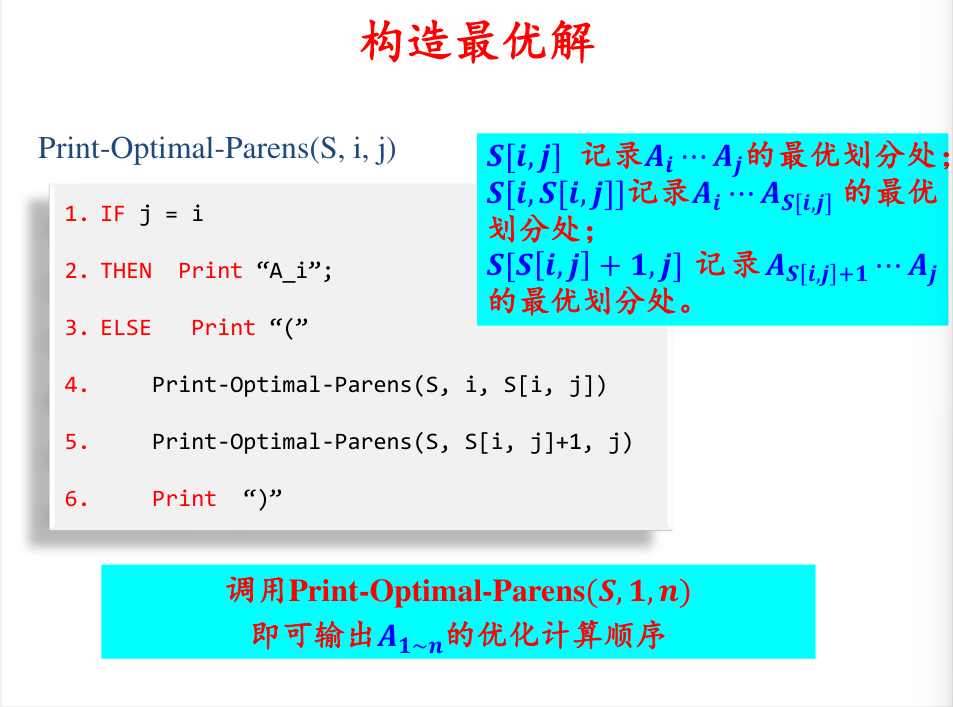
\includegraphics[scale = 0.5]{9.png}
\end{figure}
the algorithm above is very neat.
\subsection{算法复杂性}
时间复杂度: 初始化对角线, 一层循环; 然后计算上三角, 元素总共有 $\Theta \left(n ^{2}\right)$ 这么多
每个元素也要有 $\Theta \left(n\right)$ 次比较, 于是就是 $\Theta \left(n^{3}\right)$
\\根据数组 $s$ 给出最优解的构造, 需要 $\Theta \left(n\right)$, 总的就是 $\Theta \left(n ^{3}\right)$

空间复杂度: 需要用到一维向量 $p$ 来储存矩阵的行数列数, $m$ 二维矩阵来储存子问题的解, $s$ 来构造最优解, 于是空间复杂度就是 $\Theta \left(n^{2}\right)$

\begin{figure}[H]
    \centering
    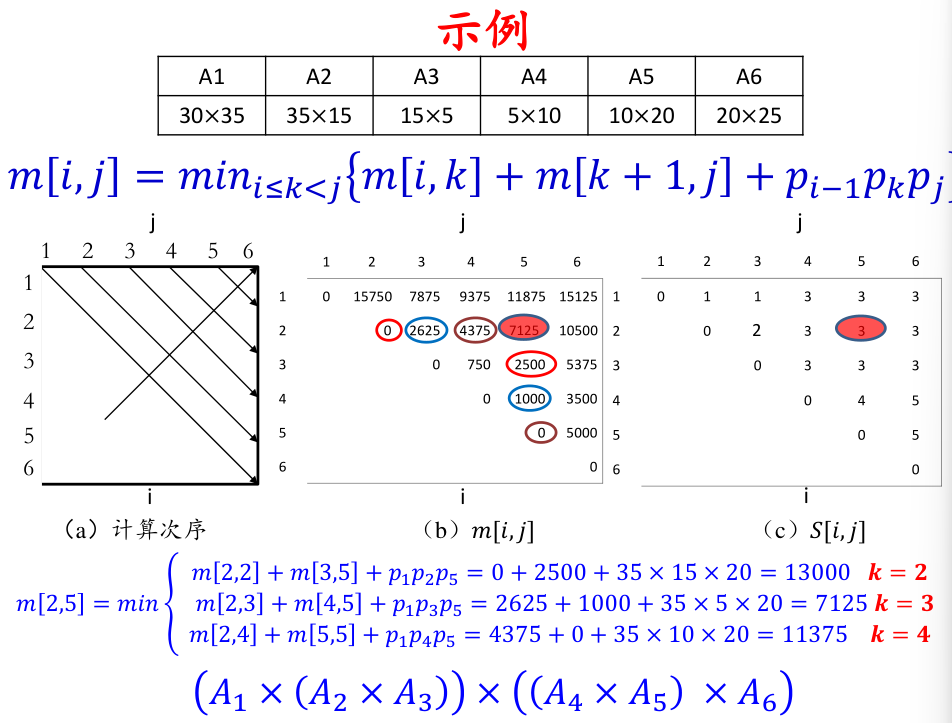
\includegraphics[scale =0.5]{10.png}
\end{figure}
\section{最长公共子序列}
比如说我们使用最长公共子序列的长度来描述两个DNA片段的相似程度
\subsection{问题描述}
\begin{definition}[subsequence]
    一个sequence $a_1,a_2,a_3,\cdots ,a_n$ 的subsequence是 $a_{i_1}, a_{i_2}, \cdots  , a_{i_k}$, 其中满足 \[i_1 < i_2 < \cdots  < i_k\footnote{和数列的子列一样}\]
\end{definition}
\begin{definition}[Common subsequence]
    对于两个序列 $A, B$, 其公共子序列 $C$ 既是 $A$ 的 subsequence 又是 $B$ 的 subsequence
\end{definition}

\noindent 问题定义: \\
输入: 两个 sequence $X = \left(x_1, x_2,\cdots , x_m\right)$ , $Y = \left(y_1, y_2, \cdots  , y_n\right)$\\
输出: 最长的公共子序列 $Z$ 

如果使用暴力求解的话, 时间复杂度将会是指数级别的, 接下来我们分析其能够使用动态规划来解决

\subsection{分析优化解的结构}
\begin{definition}
    $X$ 是一个 sequence, $\left(x_1, x_2, \cdots  ,x_i\right), i \le n$ 这个子序列称为是 $X$ 的第 $i$ 前缀, 记为 $X_{i}$
\end{definition}
\begin{theorem}[优化子结构]
    给定两个 sequence , $X = \left(x_1, \cdots  x_m\right)$, $Y = \left(y_1 , \cdots  ,y_n\right)$
    $Z= \left(z_1, \cdots  ,z_k\right)$ 是 LCS, 我们有:

    (1) 如果 $x_m = y_n$, 那么 $z_k =x_m = y_n$, $Z _{k-1}$ 是 $X _{m-1} , Y _{n-1}$ 的LCS

    (2) 如果 $x_m \ne y_n $, 且 $z_k \ne x_m$, 则 $Z$ 是 $X _{m-1 }$ 和 $Y$ 的LCS 

    (3) 如果 $x_m \ne y_n$, 且 $z_k \ne y_n$, 则 $Z$ 是 $X$ , $Y _{n-1}$ 的 LCS
\end{theorem}

证明显然, 请读者自证\footnote{Q: 为什么证明常常需要使用反证法?}

于是我们就有:
\[
LCS _{XY} = 
\begin{cases}
    LCS_{X _{m-1}Y_{n-1}} + \left(x_m\right) & x_m = y_n\\
    LCS _{X_{m-1}Y}  & x_m \ne y_n , z_k \ne x_m\\
    LCS _{X Y_{n-1}} & x_m \ne y_n , z_k \ne y_n
\end{cases}
\]

子问题具有重叠性\footnote{这时dp的基本前提, 当然这是废话}:
\begin{figure}[H]
    \centering
    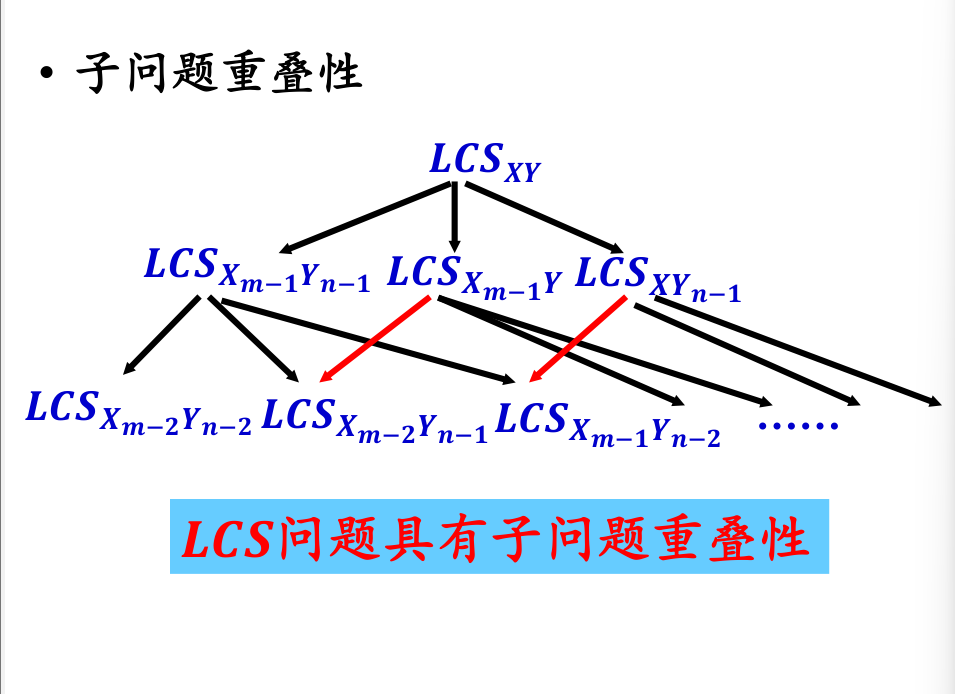
\includegraphics[scale = 0.5]{11.png}
\end{figure}
\subsection{确定递归解}
就是由上面的那个式子而来, 设 $c [i, j]$ 是前缀 $X_{i}, Y_{j}$ 的LCS的长度. 
给出LCS的长度的递归方程:
\[
c[i,j] = 
\begin{cases}
    0 &, i= 0  \text{ or } j = 0 \\
    c[i-1, j-1] + 1 & , i, j > 0, x_i = y_j\footnotemark\\
    \max \left(c \left[ i, j-1 \right], c \left[ i -1, j \right]\right) & , 
    x_i \ne y_j
\end{cases}
\]
\footnotetext{这里的ppt上有错误}
\subsubsection*{计算过程}
\begin{figure}[H]
    \centering
    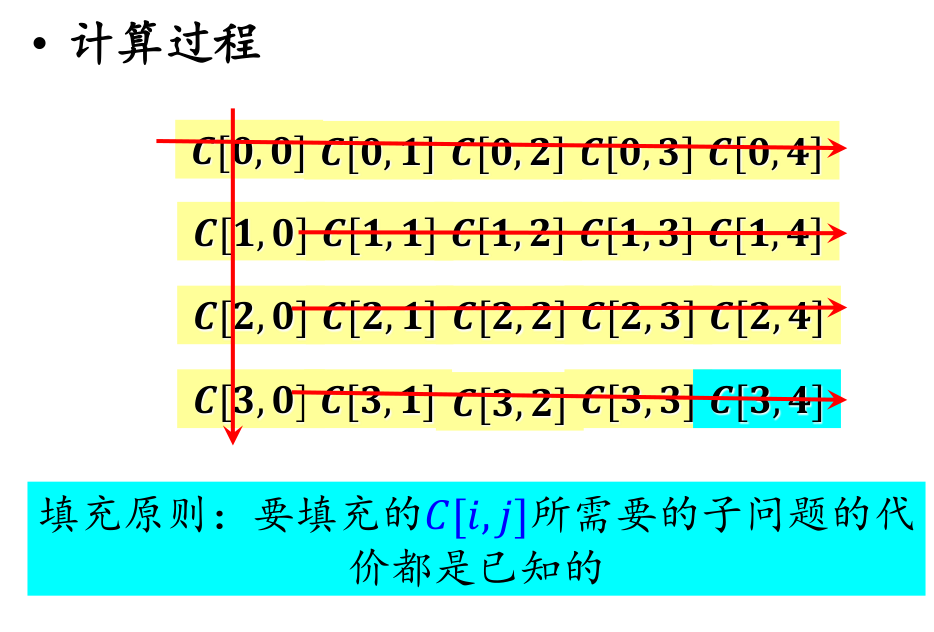
\includegraphics[scale =0.5]{12.png}
\end{figure}

先是将含有 $0$ 的求出来, 然后再一行一行地进行求解. 建议画一个表格自己进行实践.

\subsection{构造最优解}
使用一个矩阵 $b$ 来存储移动的操作, $\nwarrow$, $\gets$, $\uparrow$.
比如说, $c[i-1, j], c\left[ i, j-1 \right]$ 如果说前者是更大的, 那么就是行数减一, 就是向上 $\uparrow$
\subsection{伪代码}
\begin{figure}[H]
    \centering
    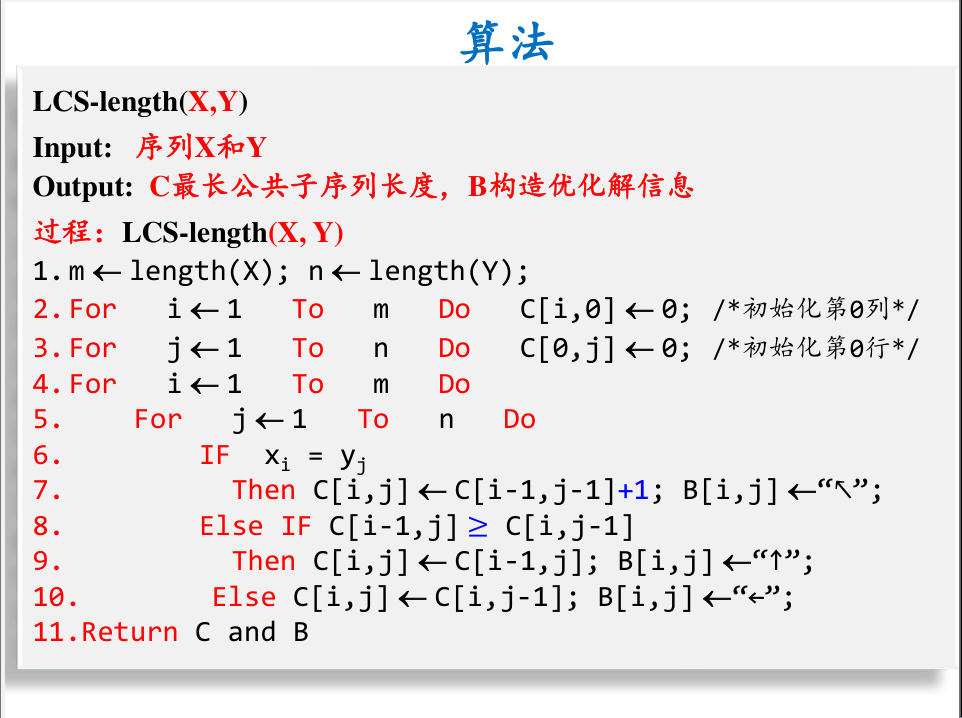
\includegraphics[scale =0.5]{13.png}
    \caption{LCS算法的伪代码}
\end{figure}
值得注意的是, 这里的箭头方向, 我们画箭头, 比较的是当前的格子和上面, 以及下面的格子.
箭头指向的方向是那个比较大的格子. 当这两个格子的值都相同的时候, 这就默认指向上方. 你得知道, 这里
箭头的方向其实是无所谓的.
\subsection{复杂度分析}
明显是 $\Theta \left(n ^{2}\right)$, 挺简单的
\subsection{最优解的构造}
读者不妨自己先思考一下, 什么时候打印出 $z$ 的某一个项

好了就当你思考完了, 反正我没思考, 我直接看到答案所以没什么办法

基本思想: 从 $b \left[ m,n \right]$ 开始, 顺着其箭头移动, 
如果说 $b\left[ i , j \right]$ 是 $\nwarrow$ 的话, 就打印出当前值.

使用递归函数能够很好地打印出来


\begin{minted}[mathescape, 
                linenos, 
                numbersep=5pt,
                gobble=2,
                frame=lines,
                framesep=2mm]{c++}
   print-LCS (b , X, i ,j){
        if (i = 0 || j = 0)
            return ;
        if (b[i, j ] = "nearrow") { //焯, 不能用数学公式啊, 这是代码
            print-LCS (b , X , i-1, j-1);
            printf (x[i]);
        }
        else if (b[i,j] = "uparrow"){ //就是向上移动, 那必然是行号减一
            print-LCS  (b , X , i-1, j);
        }else 
            print-LCS (b ,X, i , j-1); //就是向左移动, 就是列数减一
    }
\end{minted}
\section{0-1 背包问题}
这边介绍一点之后就直接进入正题好吧.

背包问题可以分为两类, 一类称为是 unbounded 背包问题, 另一类就是这里的 0-1 背包问题. 
前者是说, 一个物品的数量并没有限制, 后者中, 物品最多拿一个. 

背包问题是一种整数规划问题, 属于运筹学的学科范畴\footnote{此范畴非彼范畴}
\subsection{问题描述, 符号约定}
给定了 $n$ 种物品和一个背包, 第 $i$ 个物品的重量是 $w_{i}$, 价值是 $v_i$, 背包的容量是 $c$ (c for capacity).

问如何选择物品, 使得能装下的物品价值之和最大. 即

\[
\sum_{i \in \alpha} v_i 
\]
最大. 
有限制条件
\[
\sum_{i\in \alpha} w_i \le c
\]
其中 $\alpha$ 是一个指标集, 当然是 $\left\{1,2,\cdots ,n\right\}$ 的一个子集. 我们要求这个指标集

实际上, 对于完全背包问题, 我们已经解决了, 使用类似于矩阵链乘法的算法类似的思想就能解决.
那么为什么这个0-1背包问题不能使用相同的方法呢?
\subsection{分析优化解的结构}
\subsubsection{一个尝试}
我们根据背包的容量来划分子问题: 先是解出小背包的解, 然后再考虑大背包的. 如果说小背包的解能够用于大背包的解, 那么这个方法就是行得通的.

为什么这种方法是不行的? But this works for unbounded knapsack.
\begin{figure}[H]
    \centering
    
\includegraphics[scale =0.5]{14.png}
    \caption{为什么不行?}
\end{figure}
That is to say that we lack some information,
viz. the information of what items are used. 
But in this way the memory seem to be very weird. Because
are YOU going to list all the situation of how items are selected?
There is $\binom{n}{m}$ kind of combination if $m$ items are selected.
\subsubsection{正解}
One index is not enough if we want to divide problem.

我们通过物品的种类数量来划分子问题. 对于物品 $i$ , 
最优解只有两种情况: 没有选择 $i$ 或者选择了 $i$.
另一方面我们还是需要记录背包的容量, 以此来构造子问题. 

\begin{definition}
    $j$ 个物品, $x$ 容量的包, 其最大价值记为 $k [x  , j]$
\end{definition}

很神奇的一点就是这个和上面LCS有一些类似, 希望我们能够从其中找到一些规律

\begin{enumerate}
    \item 
    case1: 物品 $j$ 没有选择, 就有
    $k [x ,j ] = k \left[  x , j -1\right]$ 
    这是肯定的嘛, 毕竟 $j$ 没用到. 
    \item
    case2: 物品 $j$ 选择了, 就有
    $k\left[ x , j \right] =  k\left[ x - w_j,  j-1\right] + v_j$
    其中\footnote{回顾一下符号} $w_j$ 代表物品 $j$ 的重量, $v_j$ 代表物品 $j$ 的价值.
\end{enumerate}
于是综合一下就是:
\[
k\left[ x , j \right] = 
\begin{cases}
    \max \left\{ k[x,j -1], k\left[x -w_j , j-1\right] +v_j\right\} & j \ne 0 , x \ne 0\\
    0 & j = 0 \text{ or } x = 0
\end{cases}
\]
$k\left[ x, j \right]$ 中的 $x$ 不能小于 $0$ . 

\subsection{优化子结构}
\begin{definition}[a pure math description of 0-1 knap]
    \begin{description}
        \item[input] $C >0 $ , $w_{i} >0$ , $v _{i} > 0$, $1 \le i\le n$
        \item[output] $(\left(x_{1 }, x_2 ,\cdots ,x_{n}\right)), x_{i} \in \left\{ 0 ,1\right\}$ have that 
        \begin{align*}
            \sum_{1 \le i \le n}  w_{i} x_{i} \le C
        \end{align*}
        meanwhile $\displaystyle \sum_{1 \le i \le n}  v_{i}x_{i}$ is at maximum.
    \end{description}
\end{definition}
\begin{theorem}[optimal subproblem solution]
    $\left( y_1 , y_2 , \cdots  , y_{n}\right)$ is the solution to the original 0-1 problem.
    then $\left( y_1 , y_2 ,\cdots ,y_{n-1}\right)$ is a solution suit that:
    \begin{align*}
        \begin{cases}
            \displaystyle \sum_{1 \le i \le n -1}  w_{i} x_{i} \le C - w_{n} y_{n}\\
            \displaystyle \sum_{1 \le i \le n-1}  v_{i} x_{i} \text{is at maximum}\\
            x_{i} \in \left\{  0 ,1\right\} & \left( 1\le i \le n - 1\right)
        \end{cases}
    \end{align*}
\end{theorem}
\subsection{递归地定义最优值的代价}
\begin{align*}
    k \left[ x \right]\left[ j \right] = 
    \begin{cases}
        0 & j = 0 \text{ or } x = 0\\
        \max_{}  \left\{
            k\left[ x \right][j-1],k[x-w_{j}][j -1]+v_{j}
        \right\} & \text{otherwise}
    \end{cases}
\end{align*}
\subsection{伪代码}
\begin{minted}[mathescape, 
                linenos, 
                numbersep=5pt,
                gobble=2,
                frame=lines,
                framesep=2mm]{c++}
     zero-one-Kaban (w, v){
         int n = v.length // v.length 就是物品之个数
         for (x = 0 ; x <= c ; x++) {
             k[x ,0] = 0;
         }
         for (j = 1; j <= n ; j++) { //这个 j 从 0 开始也不是不行, 只不过上面的已经初始化了一次了
             k[0 ,j] = 0;
         }
         for (x = 0 ; x <= c ; x++) {
             for (j = 1; j <= n ; j++){ //一个两重循环就是为了遍历这个矩阵
                k[x,j] = k[x,j-1];
                if (w_j <= x)
                    k[x,j] = max (k[x,j], k[x-w_j, j-1] + v_j);
             }
         }
         return k[c,n]
     }
\end{minted}
\subsection{获取最优值得信息}
实际上也是和 LCS 类似, 当出现了 case2 的时候就是要记录的时候

我们只需要将上面的代码中, 加入一个记录用的数组就行. 只需要注意到, 这里的 \verb|item[x,j]| 实际上是一个序列, is subset of the
sequence.
\begin{minted}[mathescape, 
                linenos, 
                numbersep=5pt,
                gobble=2,
                frame=lines,
                framesep=2mm]{c++}
     zero-one-Kaban (w, v){
         int n = v.length // v.length 就是物品之个数
         // item 是一个矩阵, 其元素是一个集合
         for (x = 0 ; x <= c ; x++) {
             k[x ,0] = 0;
         }
         for (j = 1; j <= n ; j++) { //这个 j 从 0 开始也不是不行, 只不过上面的已经初始化了一次了
             k[0 ,j] = 0;
         }
         for (x = 0 ; x <= c ; x++) {
             for (j = 1; j <= n ; j++){ //一个两重循环就是为了遍历这个矩阵
                k[x,j] = k[x,j-1];
                if (w_j <= x){
                    k[x,j] = max (k[x,j-1], k[x-w_j, j-1] + v_j);
       /*new stuff*/if (k[x-w_j, j-1] > k[x,j-1]) { //case1
                        item[x,j] = item[x-w_j , j-1] + j 
                    }
       /*new stuff*/else  //case2
                        item[x,j] = item[x,j-1];
                }
                else (w_j > x){
                    /* do case 2*/
                }
             }
         }
         return k[c,n]
     }
\end{minted}
\section{最优二叉搜索树}
\subsection{问题描述}
\begin{definition}
有给定一个序列 $K = \left< k_1, \cdots ,k_n \right>$, 有概率 $p_{i}$ 和每一个对应,  
并且有 $n+1$ 个伪关键字 $d_i$ 表示不在 $k$ 中的值, 也有概率对应着 记为 $q_i$
有: 
\[
\sum_{i=1} ^{n}p_{i} + \sum_{i=0} ^{n}q_i = 1
\]
这是因为总的概率为1
\end{definition}

我们可以对搜索代价进行一个期望值的计算.
\[
E = \sum_{i=1} ^{n} \big(d \left(k_i\right) +1\big) + \sum_{i=0} ^{n} \big(d (d_i)+ 1 \big)  q_i\footnotemark
\]
\footnotetext{为什么是深度+1呢, 访问节点个数.}

我们说这个期望值最小的数就是一个最优二叉搜索树. 当然我们也别忘了搜索树的定义: 对于一个节点, 左子树的节点的值都小于他;
右子树的节点的值都大于他. 

\subsection{递归解的结构}
Just as previous chapter, the optimal 
search tree have optimal substrutrue property. 
That is some locally optimal 
solution to subproblems can be used to construct the optimal solution to the original problem.
\begin{theorem}[optimal subproblem structure]
最优树 $T$的一个子树 $T'$ 是最优的
\end{theorem}
\begin{proof}
    略  , 应当使用反证法.
\end{proof}

我们发现这和前面学习的矩阵链乘法非常类似, 此时我们应当确定 ``以谁为节点'', 并且计算期望, 选取期望最小的那个.

我们使用 $e \left[ i,j \right]$ 来表示关键字 $k_i , \cdots  , k_j$, 以及伪关键字 $d_{i-1}, \cdots  , d_{j}$ 组成的最优树. 
先看递归的结构 
\[
e \left[ i, j  \right] = \min \{e\left[ i,r-1 \right] + e \left[ r+1 ,j\right] +w \left[ i, j \right]\}\footnotemark
\]
\footnotetext{为什么是 $r-1$ 和 $r+1$ 呢? $w\left[ i,j  \right]$是什么意思? 怎么来的?}
To be frank, this recurrence structure can be very obvious. 
And it is not difficult to figure this out.
其中 $i \le r \le j$

此时我们还有比较特殊的处理, 这是因为左子树可以完全没有关键字, 右子树也是同理:
\[
e \left[ i, i -1 \right]= q _{i-1}
\]
\begin{example}
    $e\left[ j+1,j \right] = q_{j}$, $w [ i, i-1] = q_{i-1}$ 
\end{example}

综合起来就是

\[
e \left[ i , j  \right] =
\begin{cases}
    \min _{i \le r \le j} \left\{e \left[  i ,r -1  \right]+ e \left[ r+1 , j \right] + w[i,j]\right\} & i +1 \ne j\\
    q_{i-1} & i +1 = j\\ 
\end{cases}
\]

\subsection{自底向上地计算 optimal solution}
\begin{figure}[H]
    \centering
    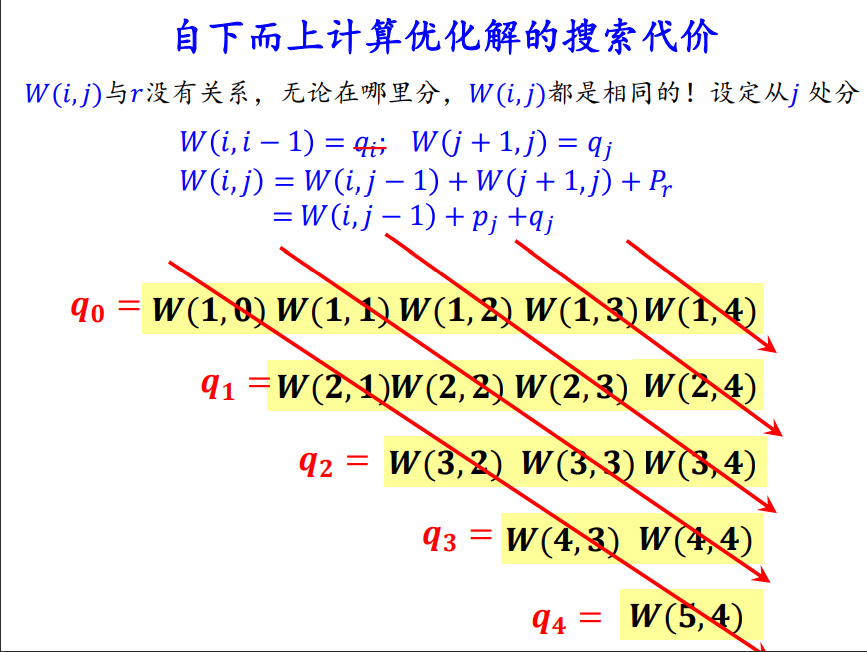
\includegraphics[scale = 0.5]{dp1.png}
\end{figure}
\begin{corollary}
    Think about how we are going to 
    write the code if 
    we want to start from diagonal.

    Also the picture above contains some mistakes.
\end{corollary}

\subsection{伪代码}
实际上求解的过程中我们还需要知道 w[i, j] 的信息, 这也可以是自底向上的计算. 
最底: $w[i, i-1] = q_{i-1    }$ 
然后
\[
w\left[ i, j \right] = w\left[ i , j-1 \right] + p_j + q_j
\]
就能求出值来

\begin{figure}[H]
    \centering
    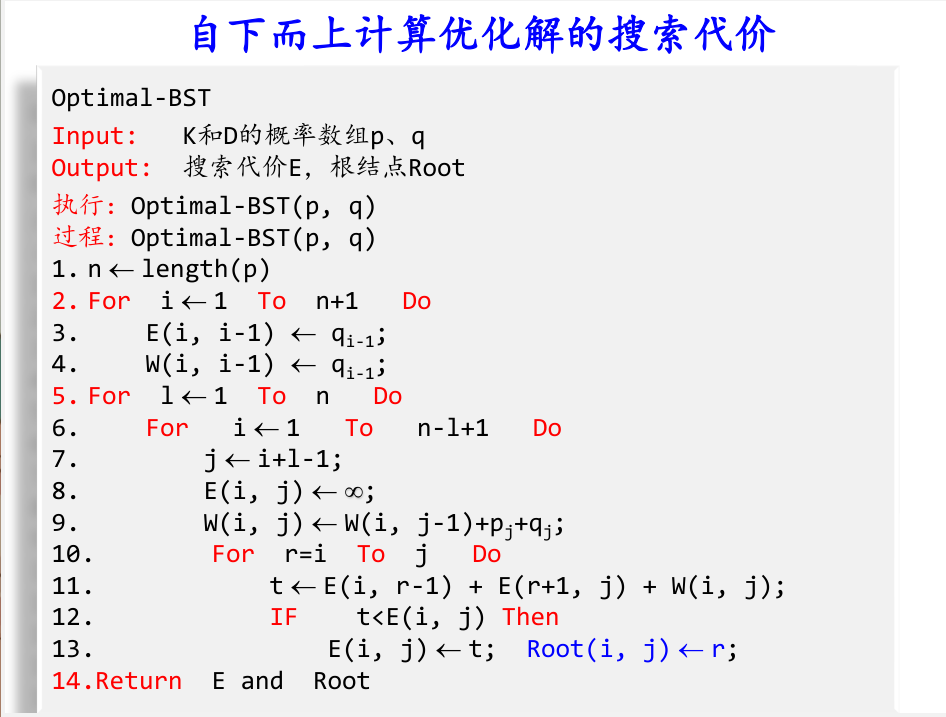
\includegraphics[scale =0.5]{15.png}
\end{figure}


\subsection{获取最优值得信息}
What we should do is to write down the 
root of nodes from $i$ to $j$, which means that 
we should use a two dimensional array.

use a 递归方法 应该就行了.

\section{Summary}
Here is Summary. At the end of the chapter, I just want to rewind, to look back,
to see what we have learnt. 

This chapter is not like the previous chapter like chapter 3. It consist of many problems that can be 
treated with dynamic programming, which may lead to that 
one get confused in those examples, whereby not understanding what dp really is.

We restate here, dynamic programming is divide and conquer plus memory. 
Moreover, the precedure to justify whether dp is a suitable approuch need us 
to 
\begin{enumerate}
    \item 
examine if the problem have optimal substrutrue, and to  
\item
examine if
the subproblems overlap during the divide and conquer approuch. 
\item
Then 
we need to figure out how to construct the
solution to bigger one basing on the solutions to subproblems \& to figure 
    
\item 
figure in which order the solution is constructed\footnote{e.g. if we start from diagonal, how we are going to write the code?}. and then to
\item 
Find a way to 获取最优值得信息, 构造最优解
\end{enumerate}
\end{document}